\subsubsection{Trong lobby}
Sơ đồ use-case trong lobby:
\begin{figure}[H]
    \centering
    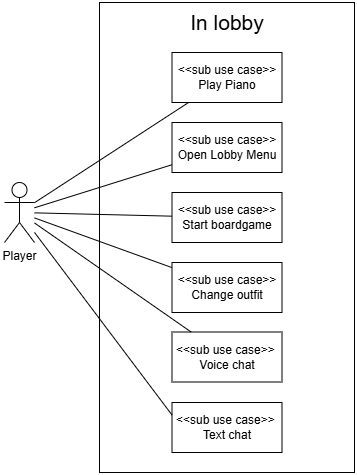
\includegraphics[width=0.75\linewidth]{4.Đặc tả chi tiết các lược đồ/Use-case/images/InLobby.png}
    \caption{Use-case mô tả trong lobby}
    \label{fig:placeholder}
\end{figure}
Người chơi có thể thực hiện các use-case phụ trong use-case trong lobby, cụ thể use-case bao gồm các use-case phụ sau:
\begin{itemize}
    \item \textbf{Chơi đàn piano}: Tại đây sẽ dẫn người chơi vào use-case Play Piano, use-case này mô tả các hoạt động cần thiết để có thể chơi được đàn piano.
    \item \textbf{Mở Lobby menu}: Tại đây sẽ dẫn người chơi vào use-case LobbyMenu, use-case này mô tả các các khả năng của người chơi khi mở Lobby Menu, bao gồm kick người chơi khác, xem thông tin phòng, ...
    \item \textbf{Bắt đầu chơi boardgame}: Tại đây sẽ dẫn người chơi vào use-case Play BoardGame, use-case này mô tả các hoạt động cần thiết để có thể vào chơi được boardgame.
    \item \textbf{Thay đổi trang phục}: Tại đây sẽ dẫn người chơi vào use-case Change Outfit, use-case này mô tả các bước cần thực hiện để có thể thay đổi được trang phục.
    \item \textbf{Voice chat}: Tại đây sẽ dẫn người chơi vào use-case Voice chat, use-case này mô tả các bước cần thực hiện để có thể sử dụng voice chat.
    \item \textbf{Text chat}: Tại đây sẽ dẫn người chơi vào use-case Text chat, use-case này mô tả các bước cần thực hiện để có thể sử dụng text chat.
\end{itemize}